\clearpage
\onecolumn
\subsection{Full Qualitative Comparison}
\label{app:qualitative-full}

% 中文：正文突出四种最有解释价值的方法；本节保留同一三个大视角样例上的完整七方法比较。
% 各列显示方法的原生输出范围，不能输出相机或场景的方法不进行人工补全。
The main paper enlarges the four comparisons most directly related to our
claim. Figure~\ref{fig:qualitative-comparison-full} retains all seven evaluated
methods on the same three transitions. Each column shows the method's available
native output; unavailable camera or scene geometry is not imputed.

\begin{center}
  \centering
  % Split the original editable vector figure into two equally scaled panels
  % so that every method remains directly comparable and legible.
  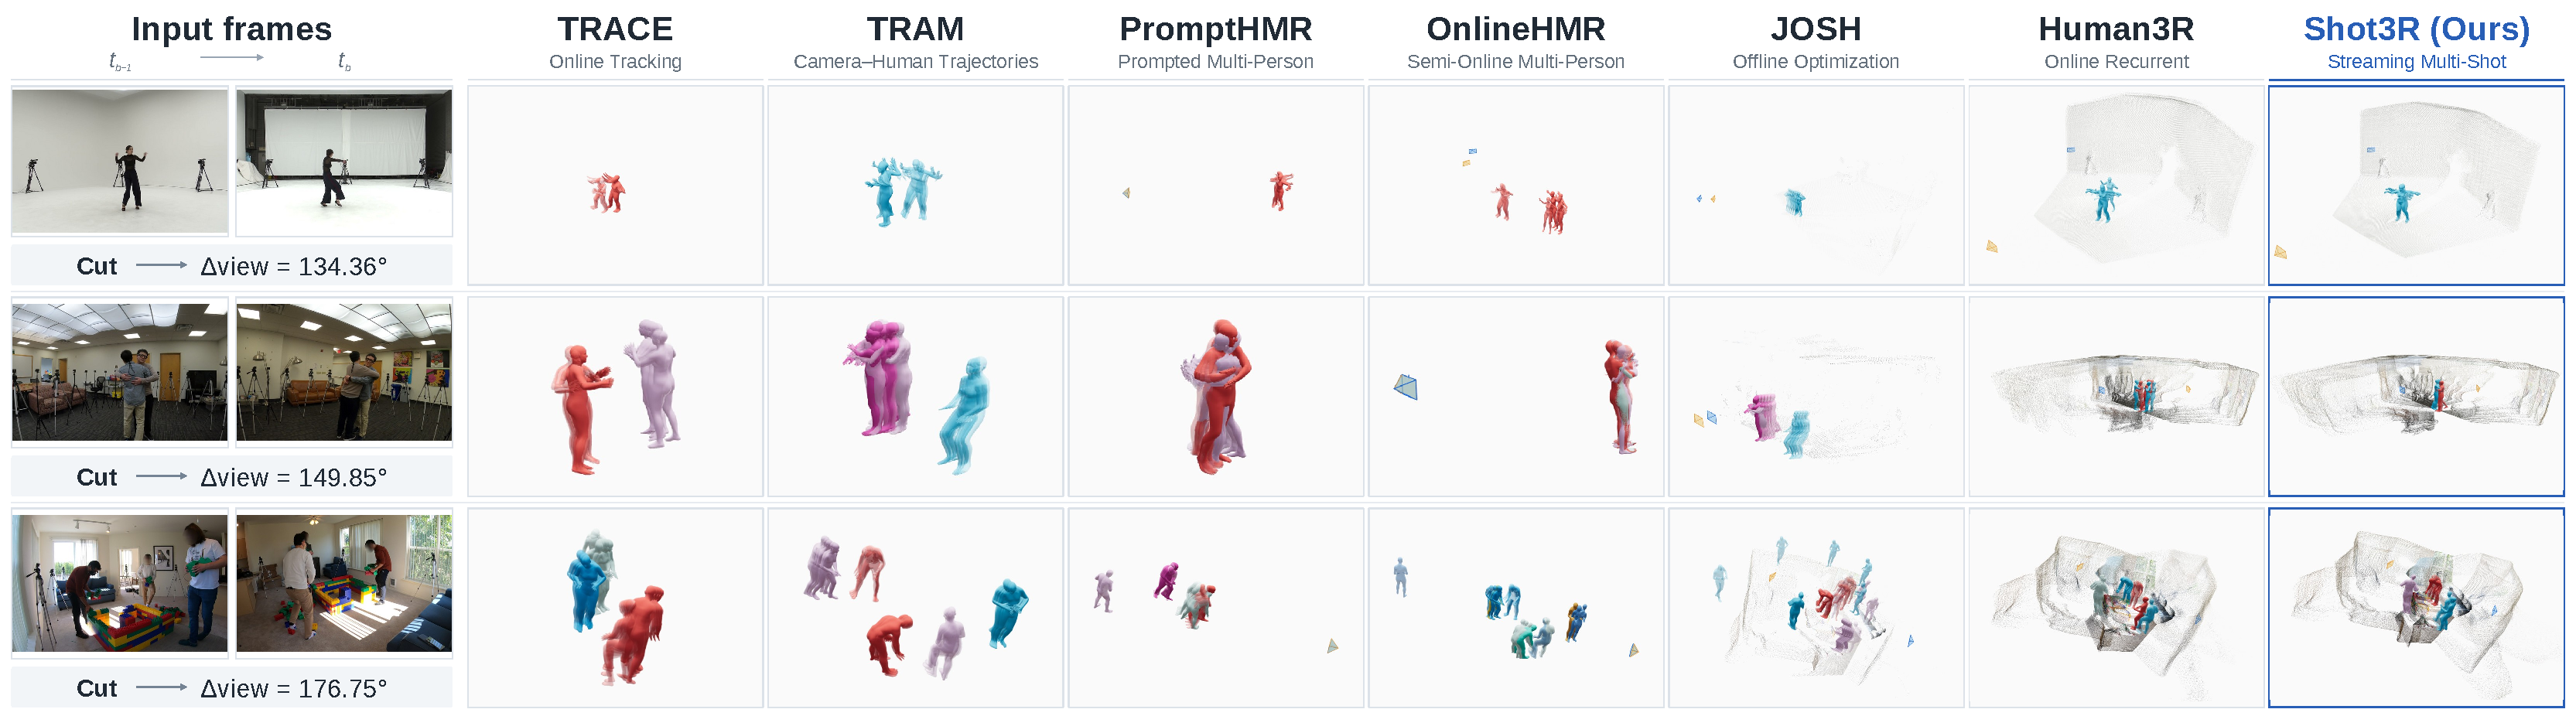
\includegraphics[width=\textwidth,trim=0pt 0pt 753pt 0pt,clip]{figures/Shot3R_qualitative_comparison.pdf}

  \vspace{4pt}
  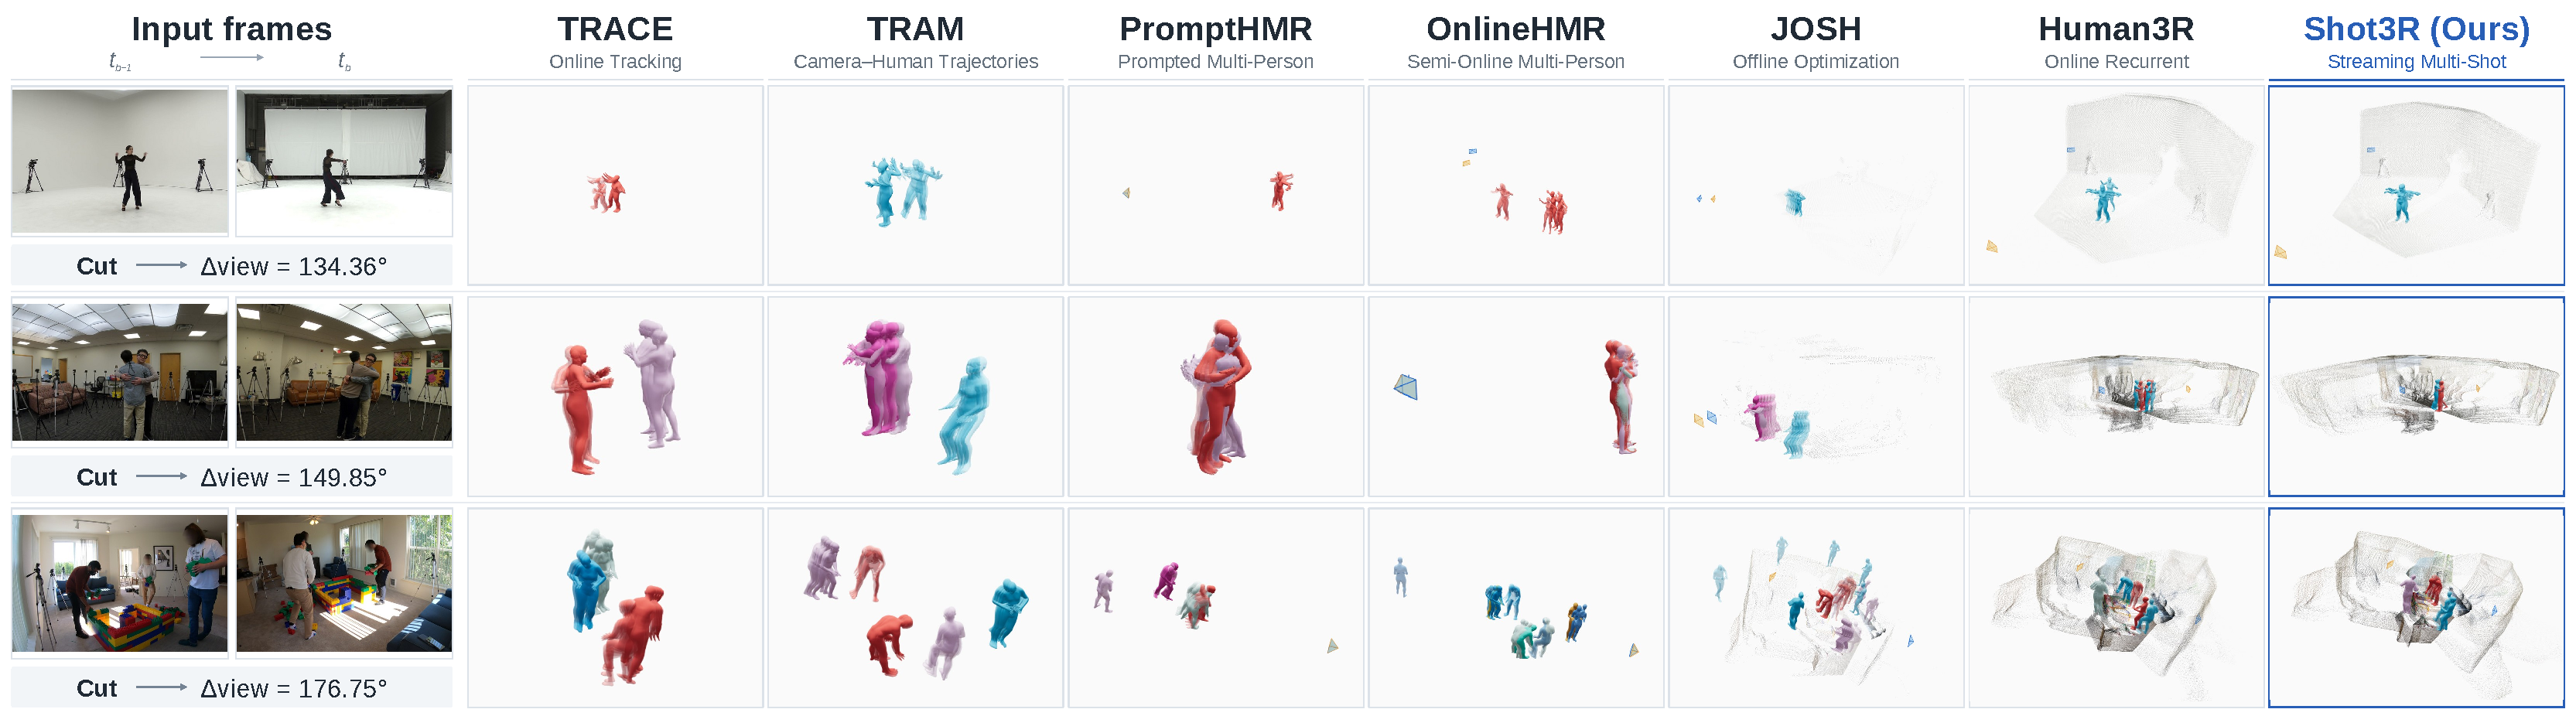
\includegraphics[width=0.891\textwidth,trim=845pt 0pt 0pt 0pt,clip]{figures/Shot3R_qualitative_comparison.pdf}
  % 中文图注：完整七方法跨镜头定性比较。视角变化从上到下为134.36、149.85和176.75度；蓝框为Shot3R。
  \captionof{figure}{\textbf{Complete qualitative comparison.} TRACE, TRAM, PromptHMR,
  OnlineHMR, JOSH, \humanthree{}, and \method{} are shown on the same inputs.
  Viewpoint changes are $134.36^\circ$, $149.85^\circ$, and $176.75^\circ$
  from top to bottom; blue borders mark \method{}.}
  \label{fig:qualitative-comparison-full}
\end{center}
\clearpage
\twocolumn
